% Options for packages loaded elsewhere
\PassOptionsToPackage{unicode}{hyperref}
\PassOptionsToPackage{hyphens}{url}
%
\documentclass[
]{article}
\usepackage{amsmath,amssymb}
\usepackage{iftex}
\ifPDFTeX
  \usepackage[T1]{fontenc}
  \usepackage[utf8]{inputenc}
  \usepackage{textcomp} % provide euro and other symbols
\else % if luatex or xetex
  \usepackage{unicode-math} % this also loads fontspec
  \defaultfontfeatures{Scale=MatchLowercase}
  \defaultfontfeatures[\rmfamily]{Ligatures=TeX,Scale=1}
\fi
\usepackage{lmodern}
\ifPDFTeX\else
  % xetex/luatex font selection
\fi
% Use upquote if available, for straight quotes in verbatim environments
\IfFileExists{upquote.sty}{\usepackage{upquote}}{}
\IfFileExists{microtype.sty}{% use microtype if available
  \usepackage[]{microtype}
  \UseMicrotypeSet[protrusion]{basicmath} % disable protrusion for tt fonts
}{}
\makeatletter
\@ifundefined{KOMAClassName}{% if non-KOMA class
  \IfFileExists{parskip.sty}{%
    \usepackage{parskip}
  }{% else
    \setlength{\parindent}{0pt}
    \setlength{\parskip}{6pt plus 2pt minus 1pt}}
}{% if KOMA class
  \KOMAoptions{parskip=half}}
\makeatother
\usepackage{xcolor}
\usepackage[margin=1in]{geometry}
\usepackage{color}
\usepackage{fancyvrb}
\newcommand{\VerbBar}{|}
\newcommand{\VERB}{\Verb[commandchars=\\\{\}]}
\DefineVerbatimEnvironment{Highlighting}{Verbatim}{commandchars=\\\{\}}
% Add ',fontsize=\small' for more characters per line
\usepackage{framed}
\definecolor{shadecolor}{RGB}{248,248,248}
\newenvironment{Shaded}{\begin{snugshade}}{\end{snugshade}}
\newcommand{\AlertTok}[1]{\textcolor[rgb]{0.94,0.16,0.16}{#1}}
\newcommand{\AnnotationTok}[1]{\textcolor[rgb]{0.56,0.35,0.01}{\textbf{\textit{#1}}}}
\newcommand{\AttributeTok}[1]{\textcolor[rgb]{0.13,0.29,0.53}{#1}}
\newcommand{\BaseNTok}[1]{\textcolor[rgb]{0.00,0.00,0.81}{#1}}
\newcommand{\BuiltInTok}[1]{#1}
\newcommand{\CharTok}[1]{\textcolor[rgb]{0.31,0.60,0.02}{#1}}
\newcommand{\CommentTok}[1]{\textcolor[rgb]{0.56,0.35,0.01}{\textit{#1}}}
\newcommand{\CommentVarTok}[1]{\textcolor[rgb]{0.56,0.35,0.01}{\textbf{\textit{#1}}}}
\newcommand{\ConstantTok}[1]{\textcolor[rgb]{0.56,0.35,0.01}{#1}}
\newcommand{\ControlFlowTok}[1]{\textcolor[rgb]{0.13,0.29,0.53}{\textbf{#1}}}
\newcommand{\DataTypeTok}[1]{\textcolor[rgb]{0.13,0.29,0.53}{#1}}
\newcommand{\DecValTok}[1]{\textcolor[rgb]{0.00,0.00,0.81}{#1}}
\newcommand{\DocumentationTok}[1]{\textcolor[rgb]{0.56,0.35,0.01}{\textbf{\textit{#1}}}}
\newcommand{\ErrorTok}[1]{\textcolor[rgb]{0.64,0.00,0.00}{\textbf{#1}}}
\newcommand{\ExtensionTok}[1]{#1}
\newcommand{\FloatTok}[1]{\textcolor[rgb]{0.00,0.00,0.81}{#1}}
\newcommand{\FunctionTok}[1]{\textcolor[rgb]{0.13,0.29,0.53}{\textbf{#1}}}
\newcommand{\ImportTok}[1]{#1}
\newcommand{\InformationTok}[1]{\textcolor[rgb]{0.56,0.35,0.01}{\textbf{\textit{#1}}}}
\newcommand{\KeywordTok}[1]{\textcolor[rgb]{0.13,0.29,0.53}{\textbf{#1}}}
\newcommand{\NormalTok}[1]{#1}
\newcommand{\OperatorTok}[1]{\textcolor[rgb]{0.81,0.36,0.00}{\textbf{#1}}}
\newcommand{\OtherTok}[1]{\textcolor[rgb]{0.56,0.35,0.01}{#1}}
\newcommand{\PreprocessorTok}[1]{\textcolor[rgb]{0.56,0.35,0.01}{\textit{#1}}}
\newcommand{\RegionMarkerTok}[1]{#1}
\newcommand{\SpecialCharTok}[1]{\textcolor[rgb]{0.81,0.36,0.00}{\textbf{#1}}}
\newcommand{\SpecialStringTok}[1]{\textcolor[rgb]{0.31,0.60,0.02}{#1}}
\newcommand{\StringTok}[1]{\textcolor[rgb]{0.31,0.60,0.02}{#1}}
\newcommand{\VariableTok}[1]{\textcolor[rgb]{0.00,0.00,0.00}{#1}}
\newcommand{\VerbatimStringTok}[1]{\textcolor[rgb]{0.31,0.60,0.02}{#1}}
\newcommand{\WarningTok}[1]{\textcolor[rgb]{0.56,0.35,0.01}{\textbf{\textit{#1}}}}
\usepackage{graphicx}
\makeatletter
\newsavebox\pandoc@box
\newcommand*\pandocbounded[1]{% scales image to fit in text height/width
  \sbox\pandoc@box{#1}%
  \Gscale@div\@tempa{\textheight}{\dimexpr\ht\pandoc@box+\dp\pandoc@box\relax}%
  \Gscale@div\@tempb{\linewidth}{\wd\pandoc@box}%
  \ifdim\@tempb\p@<\@tempa\p@\let\@tempa\@tempb\fi% select the smaller of both
  \ifdim\@tempa\p@<\p@\scalebox{\@tempa}{\usebox\pandoc@box}%
  \else\usebox{\pandoc@box}%
  \fi%
}
% Set default figure placement to htbp
\def\fps@figure{htbp}
\makeatother
\setlength{\emergencystretch}{3em} % prevent overfull lines
\providecommand{\tightlist}{%
  \setlength{\itemsep}{0pt}\setlength{\parskip}{0pt}}
\setcounter{secnumdepth}{-\maxdimen} % remove section numbering
\usepackage{bookmark}
\IfFileExists{xurl.sty}{\usepackage{xurl}}{} % add URL line breaks if available
\urlstyle{same}
\hypersetup{
  pdftitle={The relationship between unemployment and crime in the Netherlands},
  pdfauthor={Romeo Schoonderbeek, 2868407 Paul Claessens, 2859603 Furkan Kadir Öztürk, 2852640},
  hidelinks,
  pdfcreator={LaTeX via pandoc}}

\title{The relationship between unemployment and crime in the
Netherlands}
\author{Romeo Schoonderbeek, 2868407 Paul Claessens, 2859603 Furkan
Kadir Öztürk, 2852640}
\date{2025-06-24}

\begin{document}
\maketitle

\section{Set-up your environment}\label{set-up-your-environment}

\begin{Shaded}
\begin{Highlighting}[]
\FunctionTok{require}\NormalTok{(tidyverse)}
\end{Highlighting}
\end{Shaded}

\begin{verbatim}
## Loading required package: tidyverse
\end{verbatim}

\begin{verbatim}
## -- Attaching core tidyverse packages ------------------------ tidyverse 2.0.0 --
## v dplyr     1.1.4     v readr     2.1.5
## v forcats   1.0.0     v stringr   1.5.1
## v ggplot2   3.5.2     v tibble    3.3.0
## v lubridate 1.9.4     v tidyr     1.3.1
## v purrr     1.0.4     
## -- Conflicts ------------------------------------------ tidyverse_conflicts() --
## x dplyr::filter() masks stats::filter()
## x dplyr::lag()    masks stats::lag()
## i Use the conflicted package (<http://conflicted.r-lib.org/>) to force all conflicts to become errors
\end{verbatim}

\begin{Shaded}
\begin{Highlighting}[]
\FunctionTok{require}\NormalTok{(cbsodataR)}
\end{Highlighting}
\end{Shaded}

\begin{verbatim}
## Loading required package: cbsodataR
\end{verbatim}

\begin{Shaded}
\begin{Highlighting}[]
\FunctionTok{require}\NormalTok{(sf)}
\end{Highlighting}
\end{Shaded}

\begin{verbatim}
## Loading required package: sf
## Linking to GEOS 3.13.0, GDAL 3.5.3, PROJ 9.5.1; sf_use_s2() is TRUE
\end{verbatim}

\section{Part 1 - Identify a Social
Problem}\label{part-1---identify-a-social-problem}

Use APA referencing throughout your document.
\href{https://www.mendeley.com/guides/apa-citation-guide/}{Here's a link
to some explanation.}

\subsection{1.1 Describe the Social
Problem}\label{describe-the-social-problem}

Include the following:

\begin{itemize}
\item
  Why is this relevant?
\item
  \ldots{}
\end{itemize}

\section{Part 2 - Data Sourcing}\label{part-2---data-sourcing}

\subsection{2.1 Load in the data}\label{load-in-the-data}

\begin{Shaded}
\begin{Highlighting}[]
\CommentTok{\# provincelevel}
\NormalTok{DS\_Panel\_Unemployment }\OtherTok{\textless{}{-}} \FunctionTok{read.csv}\NormalTok{(}\StringTok{"data/raw\_data/unemployment\_data\_transform.csv"}\NormalTok{)}
\NormalTok{DS\_Panel\_Crime }\OtherTok{\textless{}{-}} \FunctionTok{read.csv}\NormalTok{(}\StringTok{"data/raw\_data/panel\_data\_crime.csv"}\NormalTok{)}
\NormalTok{DS\_Population }\OtherTok{\textless{}{-}} \FunctionTok{read.csv}\NormalTok{(}\StringTok{"data/population\_data.csv"}\NormalTok{)}
\NormalTok{area\_data\_working }\OtherTok{\textless{}{-}} \FunctionTok{read.csv}\NormalTok{(}\StringTok{"data/raw\_data/area\_data.csv"}\NormalTok{)}

\CommentTok{\# aggragate}

\NormalTok{agg\_unemployment }\OtherTok{\textless{}{-}} \FunctionTok{read.csv}\NormalTok{(}\StringTok{"data/raw\_data/aggragate\_total\_unemployment.csv"}\NormalTok{)}
\NormalTok{agg\_crime }\OtherTok{\textless{}{-}} \FunctionTok{read.csv}\NormalTok{(}\StringTok{"data/raw\_data/aggragate\_total\_crime.csv"}\NormalTok{)}
\NormalTok{agg\_population }\OtherTok{\textless{}{-}} \FunctionTok{read.csv}\NormalTok{(}\StringTok{"data/raw\_data/population\_data\_raw.csv"}\NormalTok{)}

\CommentTok{\# subpopulation}

\NormalTok{criminaliteit\_per\_leeftijd }\OtherTok{\textless{}{-}} \FunctionTok{read.csv}\NormalTok{(}\StringTok{"data/raw\_data/criminaliteit\_per\_leeftijd.csv"}\NormalTok{) }

\NormalTok{unemployment\_age }\OtherTok{\textless{}{-}} \FunctionTok{read.csv}\NormalTok{(}\StringTok{"data/raw\_data/unemployment\_per\_age.csv"}\NormalTok{) }
\end{Highlighting}
\end{Shaded}

\subsection{2.2 Provide a short summary of the
dataset(s)}\label{provide-a-short-summary-of-the-datasets}

In this case we see 28 variables, but we miss some information on what
units they are in. We also don't know anything about the year/moment in
which this data has been captured.

\begin{Shaded}
\begin{Highlighting}[]
\NormalTok{inline\_code }\OtherTok{=} \ConstantTok{TRUE}
\end{Highlighting}
\end{Shaded}

These are things that are usually included in the metadata of the
dataset. For your project, you need to provide us with the information
from your metadata that we need to understand your dataset of choice.

\subsection{2.3 Describe the type of variables
included}\label{describe-the-type-of-variables-included}

Think of things like:

\begin{itemize}
\item
  Do the variables contain health information or SES information?
\item
  Have they been measured by interviewing individuals or is the data
  coming from administrative sources?
\end{itemize}

\emph{For the sake of this example, I will continue with the
assignment\ldots{}}

\section{Part 3 - Quantifying}\label{part-3---quantifying}

\subsection{3.1 Data cleaning}\label{data-cleaning}

CBS datasets already come in panel data form. Data cleaning will include
removing unnecessary rows and columns, adjusting data frames and merging
data sets. 3 main data sets are used. Province panel data, aggregate
panel data and data sets used for sub population analysis.

\begin{Shaded}
\begin{Highlighting}[]
\CommentTok{\# province panel data cleaning}

\NormalTok{merged\_data }\OtherTok{\textless{}{-}} \FunctionTok{cbind}\NormalTok{(DS\_Panel\_Unemployment, DS\_Panel\_Crime [, }\DecValTok{5}\NormalTok{])}

\NormalTok{merged\_data }\OtherTok{\textless{}{-}}\FunctionTok{cbind}\NormalTok{(merged\_data, DS\_Population [, }\DecValTok{4}\NormalTok{])}

\NormalTok{merged\_data }\OtherTok{\textless{}{-}}\NormalTok{ merged\_data [, }\SpecialCharTok{{-}}\FunctionTok{c}\NormalTok{(}\DecValTok{1}\NormalTok{)] }
\FunctionTok{colnames}\NormalTok{(merged\_data) }\OtherTok{\textless{}{-}} \FunctionTok{c}\NormalTok{(}\StringTok{"Year"}\NormalTok{, }\StringTok{"province"}\NormalTok{, }\StringTok{"Unemployment\_Rate"}\NormalTok{, }\StringTok{"total\_Crimes"}\NormalTok{, }\StringTok{"Population"}\NormalTok{)}

\NormalTok{merged\_data }\OtherTok{\textless{}{-}} \FunctionTok{mutate}\NormalTok{(merged\_data, }\AttributeTok{crimes\_per\_capita =}\NormalTok{ (total\_Crimes}\SpecialCharTok{/}\NormalTok{Population)}\SpecialCharTok{*}\DecValTok{100}\NormalTok{)}

\FunctionTok{write.csv}\NormalTok{(merged\_data, }\StringTok{"data/working\_data/merged\_panel\_data\_final.csv"}\NormalTok{)}

\NormalTok{area\_data\_working }\OtherTok{\textless{}{-}} \FunctionTok{read.csv}\NormalTok{(}\StringTok{"data/raw\_data/area\_data.csv"}\NormalTok{)}

\FunctionTok{colnames}\NormalTok{(area\_data\_working) }\OtherTok{=} \FunctionTok{c}\NormalTok{(}\StringTok{"X"}\NormalTok{, }\StringTok{"province"}\NormalTok{, }\StringTok{"Area(KM2)"}\NormalTok{)}

\NormalTok{area\_data\_working }\OtherTok{\textless{}{-}}\NormalTok{ area\_data\_working[}\DecValTok{6}\SpecialCharTok{:}\DecValTok{17}\NormalTok{ ,]}

\NormalTok{area\_data\_working[[}\DecValTok{3}\NormalTok{]]  }\OtherTok{=} \FunctionTok{as.numeric}\NormalTok{(area\_data\_working[[}\DecValTok{3}\NormalTok{]])}

\NormalTok{area\_data\_working[, }\DecValTok{3}\NormalTok{] }\OtherTok{=}\NormalTok{ area\_data\_working[, }\DecValTok{3}\NormalTok{]}\SpecialCharTok{/} \DecValTok{100}

\NormalTok{flevoland }\OtherTok{\textless{}{-}} \FunctionTok{data.frame}\NormalTok{(}\AttributeTok{name =} \StringTok{"Flevoland"}\NormalTok{, }\AttributeTok{value =} \DecValTok{1417}\NormalTok{ )}
\FunctionTok{colnames}\NormalTok{(flevoland) }\OtherTok{=} \FunctionTok{c}\NormalTok{(}\StringTok{"province"}\NormalTok{, }\StringTok{"Area(KM2)"}\NormalTok{)}

\NormalTok{area\_data\_working }\OtherTok{\textless{}{-}} \FunctionTok{bind\_rows}\NormalTok{(}
\NormalTok{  area\_data\_working[}\DecValTok{1}\SpecialCharTok{:}\DecValTok{5}\NormalTok{, ], flevoland,  }
\NormalTok{  area\_data\_working[}\DecValTok{6}\SpecialCharTok{:}\FunctionTok{nrow}\NormalTok{(area\_data\_working), ]}
\NormalTok{)}
\end{Highlighting}
\end{Shaded}

\begin{verbatim}
## New names:
## New names:
## * `` -> `...4`
## * `` -> `...5`
## * `` -> `...6`
\end{verbatim}

\begin{Shaded}
\begin{Highlighting}[]
\NormalTok{area\_data\_working }\OtherTok{\textless{}{-}}\NormalTok{ area\_data\_working }\SpecialCharTok{\%\textgreater{}\%}
  \FunctionTok{slice}\NormalTok{(}\FunctionTok{rep}\NormalTok{(}\DecValTok{1}\SpecialCharTok{:}\FunctionTok{n}\NormalTok{(), }\AttributeTok{each =} \DecValTok{12}\NormalTok{))}

\NormalTok{merged\_panel\_data\_final }\OtherTok{\textless{}{-}} \FunctionTok{cbind}\NormalTok{(merged\_data, area\_data\_working[, }\DecValTok{3}\NormalTok{])}

\FunctionTok{colnames}\NormalTok{(merged\_panel\_data\_final) }\OtherTok{\textless{}{-}} \FunctionTok{c}\NormalTok{(}\StringTok{"year"}\NormalTok{, }\StringTok{"province"}\NormalTok{, }\StringTok{"unemployment\_rate"}\NormalTok{, }\StringTok{"total\_crimes"}\NormalTok{, }\StringTok{"population"}\NormalTok{, }\StringTok{"crimes\_per\_capita"}\NormalTok{, }\StringTok{"area\_km2"}\NormalTok{)}

\NormalTok{merged\_panel\_data\_final }\OtherTok{\textless{}{-}} \FunctionTok{mutate}\NormalTok{(merged\_panel\_data\_final, }\AttributeTok{poplation\_density =}\NormalTok{ population}\SpecialCharTok{/}\NormalTok{area\_km2)}

\CommentTok{\# aggregate data cleaning}

\NormalTok{agg\_unemployment }\OtherTok{\textless{}{-}}\NormalTok{ agg\_unemployment[}\SpecialCharTok{{-}}\FunctionTok{c}\NormalTok{(}\DecValTok{51}\NormalTok{,}\DecValTok{52}\NormalTok{) ,]}
\NormalTok{agg\_unemployment }\OtherTok{\textless{}{-}}\NormalTok{ agg\_unemployment[, }\SpecialCharTok{{-}}\DecValTok{1}\NormalTok{]}

\NormalTok{agg\_crime }\OtherTok{\textless{}{-}}\NormalTok{ agg\_crime[}\SpecialCharTok{{-}}\DecValTok{82}\NormalTok{ , ]}
\NormalTok{agg\_crime }\OtherTok{\textless{}{-}}\NormalTok{ agg\_crime[}\SpecialCharTok{{-}}\FunctionTok{c}\NormalTok{(}\DecValTok{1}\SpecialCharTok{:}\DecValTok{31}\NormalTok{) ,]}
\NormalTok{agg\_crime }\OtherTok{\textless{}{-}}\NormalTok{ agg\_crime[, }\SpecialCharTok{{-}}\DecValTok{1}\NormalTok{]}

\FunctionTok{colnames}\NormalTok{(agg\_unemployment) }\OtherTok{=} \FunctionTok{c}\NormalTok{(}\StringTok{"year"}\NormalTok{, }\StringTok{"unemployment"}\NormalTok{)}
\FunctionTok{colnames}\NormalTok{(agg\_crime) }\OtherTok{=} \FunctionTok{c}\NormalTok{(}\StringTok{"year"}\NormalTok{, }\StringTok{"total\_crimes"}\NormalTok{)}

\NormalTok{agg\_merged }\OtherTok{\textless{}{-}} \FunctionTok{cbind}\NormalTok{(agg\_unemployment, agg\_crime[, }\DecValTok{2}\NormalTok{])}

\FunctionTok{colnames}\NormalTok{(agg\_merged) }\OtherTok{=} \FunctionTok{c}\NormalTok{(}\StringTok{"year"}\NormalTok{, }\StringTok{"unemployment"}\NormalTok{, }\StringTok{"total\_crime"}\NormalTok{)}

\NormalTok{agg\_merged }\OtherTok{\textless{}{-}}\NormalTok{ agg\_merged }\SpecialCharTok{\%\textgreater{}\%}
  \FunctionTok{mutate}\NormalTok{(}\AttributeTok{total\_crime =} \FunctionTok{as.numeric}\NormalTok{(total\_crime)) }\SpecialCharTok{\%\textgreater{}\%}
  \FunctionTok{mutate}\NormalTok{(}\AttributeTok{year =} \FunctionTok{as.numeric}\NormalTok{(year))}

\FunctionTok{str}\NormalTok{(agg\_merged)}
\end{Highlighting}
\end{Shaded}

\begin{verbatim}
## 'data.frame':    50 obs. of  3 variables:
##  $ year        : num  1975 1976 1977 1978 1979 ...
##  $ unemployment: num  3.5 4.2 4.3 4.2 4.1 4.3 5.7 8 9.6 9.6 ...
##  $ total_crime : num  486670 564025 590880 612370 668235 ...
\end{verbatim}

\begin{Shaded}
\begin{Highlighting}[]
\NormalTok{agg\_population }\OtherTok{\textless{}{-}}\NormalTok{agg\_population[, }\SpecialCharTok{{-}}\DecValTok{4}\NormalTok{]}
\NormalTok{agg\_population }\OtherTok{\textless{}{-}}\NormalTok{ agg\_population[, }\SpecialCharTok{{-}}\DecValTok{1}\NormalTok{]}
\NormalTok{agg\_population }\OtherTok{\textless{}{-}}\NormalTok{ agg\_population[}\SpecialCharTok{{-}}\FunctionTok{c}\NormalTok{(}\DecValTok{1}\SpecialCharTok{:}\DecValTok{75}\NormalTok{) ,]}

\NormalTok{agg\_merged }\OtherTok{\textless{}{-}} \FunctionTok{cbind}\NormalTok{(agg\_merged, agg\_population[, }\DecValTok{2}\NormalTok{])}

\FunctionTok{colnames}\NormalTok{(agg\_merged) }\OtherTok{=} \FunctionTok{c}\NormalTok{(}\StringTok{"year"}\NormalTok{, }\StringTok{"unemployment"}\NormalTok{, }\StringTok{"total\_crime"}\NormalTok{, }\StringTok{"population"}\NormalTok{)}

\FunctionTok{str}\NormalTok{(agg\_merged)}
\end{Highlighting}
\end{Shaded}

\begin{verbatim}
## 'data.frame':    50 obs. of  4 variables:
##  $ year        : num  1975 1976 1977 1978 1979 ...
##  $ unemployment: num  3.5 4.2 4.3 4.2 4.1 4.3 5.7 8 9.6 9.6 ...
##  $ total_crime : num  486670 564025 590880 612370 668235 ...
##  $ population  : int  13600000 13730000 13810000 13900000 13990000 14090000 14210000 14290000 14340000 14400000 ...
\end{verbatim}

\begin{Shaded}
\begin{Highlighting}[]
\NormalTok{agg\_merged }\OtherTok{\textless{}{-}}\NormalTok{ agg\_merged }\SpecialCharTok{\%\textgreater{}\%}
  \FunctionTok{mutate}\NormalTok{(}\AttributeTok{crime\_per\_capita =}\NormalTok{ (total\_crime}\SpecialCharTok{/}\NormalTok{population)}\SpecialCharTok{*}\DecValTok{100}\NormalTok{)}

\CommentTok{\# subpopulation}

\NormalTok{crime2021 }\OtherTok{\textless{}{-}}\NormalTok{ criminaliteit\_per\_leeftijd }\SpecialCharTok{\%\textgreater{}\%} \FunctionTok{filter}\NormalTok{(Perioden }\SpecialCharTok{==} \StringTok{"2021"}\NormalTok{)}

\NormalTok{crime2021 }\OtherTok{\textless{}{-}}\NormalTok{ crime2021 }\SpecialCharTok{\%\textgreater{}\%} \FunctionTok{filter}\NormalTok{(Geboorteland }\SpecialCharTok{==} \StringTok{"Totaal"}\NormalTok{)}

\NormalTok{columns }\OtherTok{\textless{}{-}} \FunctionTok{c}\NormalTok{(}\StringTok{"Leeftijdscategorie"}\NormalTok{, }\StringTok{"PercCriminilateit"}\NormalTok{)}

\NormalTok{eindproduct }\OtherTok{\textless{}{-}}\NormalTok{ columns}

\NormalTok{crime2021 }\OtherTok{\textless{}{-}}\NormalTok{ crime2021[, }\SpecialCharTok{{-}}\FunctionTok{c}\NormalTok{(}\DecValTok{1}\SpecialCharTok{:}\DecValTok{2}\NormalTok{)]}
\NormalTok{crime2021 }\OtherTok{\textless{}{-}}\NormalTok{ crime2021[, }\SpecialCharTok{{-}}\FunctionTok{c}\NormalTok{(}\DecValTok{2}\SpecialCharTok{:}\DecValTok{6}\NormalTok{)]}

\NormalTok{unemployment\_age }\OtherTok{\textless{}{-}}\NormalTok{ unemployment\_age[}\SpecialCharTok{{-}}\FunctionTok{c}\NormalTok{(}\DecValTok{1}\SpecialCharTok{:}\DecValTok{6}\NormalTok{, }\DecValTok{19}\NormalTok{) ,]}

\NormalTok{unemployment\_age }\OtherTok{\textless{}{-}}\NormalTok{ unemployment\_age[, }\SpecialCharTok{{-}}\DecValTok{1}\NormalTok{]}

\FunctionTok{colnames}\NormalTok{(unemployment\_age) }\OtherTok{=} \FunctionTok{c}\NormalTok{(}\StringTok{"leeftijd"}\NormalTok{, }\StringTok{"unemployment"}\NormalTok{)}
\end{Highlighting}
\end{Shaded}

Please use a separate `R block' of code for each type of cleaning. So,
e.g.~one for missing values, a new one for removing unnecessary
variables etc.

\subsection{3.2 Generate necessary
variables}\label{generate-necessary-variables}

Variable 1

Variable 2

\begin{Shaded}
\begin{Highlighting}[]
\NormalTok{crime2021}\SpecialCharTok{$}\NormalTok{Leeftijd }\OtherTok{\textless{}{-}} \FunctionTok{ifelse}\NormalTok{(crime2021}\SpecialCharTok{$}\NormalTok{Leeftijd }\SpecialCharTok{\%in\%} \FunctionTok{c}\NormalTok{(}\StringTok{"12 tot 18 jaar"}\NormalTok{, }\StringTok{"18 tot 23 jaar"}\NormalTok{),}
                                     \StringTok{"Youth (12–23)"}\NormalTok{, }\StringTok{"Adult+ (23+)"}\NormalTok{)}

\FunctionTok{colnames}\NormalTok{(crime2021) }\OtherTok{=} \FunctionTok{c}\NormalTok{(}\StringTok{"leeftijdcat"}\NormalTok{, }\StringTok{"crime"}\NormalTok{)}

\NormalTok{unemployment\_age}\SpecialCharTok{$}\NormalTok{leeftijd }\OtherTok{\textless{}{-}} \FunctionTok{ifelse}\NormalTok{(unemployment\_age}\SpecialCharTok{$}\NormalTok{leeftijd }\SpecialCharTok{\%in\%} \FunctionTok{c}\NormalTok{(}\StringTok{"15 tot 20 jaar"}\NormalTok{, }\StringTok{"20 tot 25 jaar"}\NormalTok{),}
                             \StringTok{"Youth"}\NormalTok{, }\StringTok{"Adult"}\NormalTok{)}

\NormalTok{unemployment\_age}\SpecialCharTok{$}\NormalTok{unemployment }\OtherTok{\textless{}{-}} \FunctionTok{gsub}\NormalTok{(}\StringTok{","}\NormalTok{, }\StringTok{"."}\NormalTok{, unemployment\_age}\SpecialCharTok{$}\NormalTok{unemployment)}

\CommentTok{\# Convert character to numeric}
\NormalTok{unemployment\_age}\SpecialCharTok{$}\NormalTok{unemployment }\OtherTok{\textless{}{-}} \FunctionTok{as.numeric}\NormalTok{(unemployment\_age}\SpecialCharTok{$}\NormalTok{unemployment)}
\end{Highlighting}
\end{Shaded}

\subsection{3.3 Visualize temporal
variation}\label{visualize-temporal-variation}

\begin{Shaded}
\begin{Highlighting}[]
\NormalTok{pivot\_agg\_data }\OtherTok{\textless{}{-}}\NormalTok{ agg\_merged }\SpecialCharTok{\%\textgreater{}\%}
  \FunctionTok{pivot\_longer}\NormalTok{(}\AttributeTok{cols =} \FunctionTok{c}\NormalTok{(unemployment, crime\_per\_capita), }\AttributeTok{names\_to =} \StringTok{"variable"}\NormalTok{, }\AttributeTok{values\_to =} \StringTok{"value"}\NormalTok{)}

\CommentTok{\# then make the plot}

\FunctionTok{ggplot}\NormalTok{(pivot\_agg\_data, }\FunctionTok{aes}\NormalTok{(}\AttributeTok{x =}\NormalTok{ year, }\AttributeTok{y =}\NormalTok{ value, }\AttributeTok{colour =}\NormalTok{ variable )) }\SpecialCharTok{+}
  \FunctionTok{geom\_line}\NormalTok{() }\SpecialCharTok{+}
  \FunctionTok{labs}\NormalTok{(}\AttributeTok{title =} \StringTok{"aggragate crime and unemployment through time"}\NormalTok{, }\AttributeTok{x =} \StringTok{"year"}\NormalTok{, }\AttributeTok{y =} \StringTok{"variable"}\NormalTok{) }\SpecialCharTok{+}
  \FunctionTok{scale\_x\_continuous}\NormalTok{(}\AttributeTok{breaks =} \FunctionTok{seq}\NormalTok{(}\DecValTok{1975}\NormalTok{, }\DecValTok{2024}\NormalTok{, }\AttributeTok{by =} \DecValTok{5}\NormalTok{), }\AttributeTok{limits =} \FunctionTok{c}\NormalTok{(}\DecValTok{1972}\NormalTok{, }\DecValTok{2026}\NormalTok{))}
\end{Highlighting}
\end{Shaded}

\pandocbounded{\includegraphics[keepaspectratio]{experimental-dynamic-maps_files/figure-latex/unnamed-chunk-3-1.pdf}}

\subsection{3.4 Visualize spatial
variation}\label{visualize-spatial-variation}

\begin{Shaded}
\begin{Highlighting}[]
\NormalTok{cbs\_maps }\OtherTok{\textless{}{-}} \FunctionTok{cbs\_get\_maps}\NormalTok{()}
\CommentTok{\# the layout of the data.frame is:}
\FunctionTok{str}\NormalTok{(cbs\_maps)}
\end{Highlighting}
\end{Shaded}

\begin{verbatim}
## 'data.frame':    620 obs. of  4 variables:
##  $ region: chr  "arbeidsmarktregio" "arbeidsmarktregio" "arbeidsmarktregio" "arbeidsmarktregio" ...
##  $ year  : int  2014 2015 2016 2017 2018 2019 2020 2021 2022 2023 ...
##  $ wgs84 : chr  "https://cartomap.github.io/nl/wgs84/arbeidsmarktregio_2014.geojson" "https://cartomap.github.io/nl/wgs84/arbeidsmarktregio_2015.geojson" "https://cartomap.github.io/nl/wgs84/arbeidsmarktregio_2016.geojson" "https://cartomap.github.io/nl/wgs84/arbeidsmarktregio_2017.geojson" ...
##  $ rd    : chr  "https://cartomap.github.io/nl/rd/arbeidsmarktregio_2014.geojson" "https://cartomap.github.io/nl/rd/arbeidsmarktregio_2015.geojson" "https://cartomap.github.io/nl/rd/arbeidsmarktregio_2016.geojson" "https://cartomap.github.io/nl/rd/arbeidsmarktregio_2017.geojson" ...
\end{verbatim}

\begin{Shaded}
\begin{Highlighting}[]
\CommentTok{\#read the GeoJSON straight from PDOK }
\NormalTok{nl\_prov }\OtherTok{\textless{}{-}} \FunctionTok{st\_read}\NormalTok{(}
  \StringTok{"https://cartomap.github.io/nl/wgs84/provincie\_2014.geojson"}\NormalTok{,}
  \AttributeTok{quiet =} \ConstantTok{TRUE}
\NormalTok{)}
\end{Highlighting}
\end{Shaded}

\begin{Shaded}
\begin{Highlighting}[]
\CommentTok{\#Reading the CSV  →  2023 only}
\CommentTok{\# nl crime }
\NormalTok{crime }\OtherTok{\textless{}{-}}\NormalTok{ merged\_panel\_data\_final }\SpecialCharTok{|\textgreater{}}
  \FunctionTok{filter}\NormalTok{(year }\SpecialCharTok{==} \DecValTok{2023}\NormalTok{) }\SpecialCharTok{|\textgreater{}}
  \FunctionTok{mutate}\NormalTok{(}
    \AttributeTok{province =} \FunctionTok{sub}\NormalTok{(}\StringTok{" }\SpecialCharTok{\textbackslash{}\textbackslash{}}\StringTok{(PV}\SpecialCharTok{\textbackslash{}\textbackslash{}}\StringTok{)$"}\NormalTok{, }\StringTok{""}\NormalTok{, province),        }
    \AttributeTok{province =} \FunctionTok{recode}\NormalTok{(province, }\StringTok{"Fryslân"} \OtherTok{=} \StringTok{"Friesland"}\NormalTok{)}
\NormalTok{  ) }\SpecialCharTok{|\textgreater{}}
  \FunctionTok{filter}\NormalTok{(}\SpecialCharTok{!}\NormalTok{province }\SpecialCharTok{\%in\%} \StringTok{"Nederland"}\NormalTok{)}
\end{Highlighting}
\end{Shaded}

\begin{Shaded}
\begin{Highlighting}[]
\CommentTok{\# Province shapes (CBS 2014)}
\NormalTok{prov\_shapes }\OtherTok{\textless{}{-}} \FunctionTok{read\_sf}\NormalTok{(}\StringTok{"https://cartomap.github.io/nl/wgs84/provincie\_2014.geojson"}\NormalTok{)}


\CommentTok{\# Join data → map}
\NormalTok{nl\_crime }\OtherTok{\textless{}{-}}\NormalTok{ prov\_shapes }\SpecialCharTok{|\textgreater{}}
  \FunctionTok{left\_join}\NormalTok{(crime, }\AttributeTok{by =} \FunctionTok{c}\NormalTok{(}\StringTok{"statnaam"} \OtherTok{=} \StringTok{"province"}\NormalTok{))}
\end{Highlighting}
\end{Shaded}

\begin{Shaded}
\begin{Highlighting}[]
\FunctionTok{ggplot}\NormalTok{(nl\_crime) }\SpecialCharTok{+}
  \FunctionTok{geom\_sf}\NormalTok{(}\FunctionTok{aes}\NormalTok{(}\AttributeTok{fill =}\NormalTok{ crimes\_per\_capita), }\AttributeTok{color =} \StringTok{"white"}\NormalTok{, }\AttributeTok{size =} \FloatTok{0.2}\NormalTok{) }\SpecialCharTok{+}
  \FunctionTok{scale\_fill\_gradient}\NormalTok{(}
    \AttributeTok{low  =} \StringTok{"\#fee5d9"}\NormalTok{,  }\CommentTok{\# pale red}
    \AttributeTok{high =} \StringTok{"\#a50f15"}\NormalTok{,  }\CommentTok{\# dark red}
    \AttributeTok{na.value =} \StringTok{"grey90"}\NormalTok{,}
    \AttributeTok{name =} \StringTok{"Crime}\SpecialCharTok{\textbackslash{}n}\StringTok{per capita"}
\NormalTok{  ) }\SpecialCharTok{+}
  \FunctionTok{labs}\NormalTok{(}
    \AttributeTok{title =} \StringTok{"Crime per capita by Dutch province – 2023"}
\NormalTok{  ) }\SpecialCharTok{+}
  \FunctionTok{theme\_minimal}\NormalTok{() }\SpecialCharTok{+}
  \FunctionTok{theme}\NormalTok{(}
    \AttributeTok{panel.grid =} \FunctionTok{element\_blank}\NormalTok{(),}
    \AttributeTok{axis.text  =} \FunctionTok{element\_blank}\NormalTok{(),}
    \AttributeTok{axis.ticks =} \FunctionTok{element\_blank}\NormalTok{()}
\NormalTok{  )}
\end{Highlighting}
\end{Shaded}

\pandocbounded{\includegraphics[keepaspectratio]{experimental-dynamic-maps_files/figure-latex/unnamed-chunk-7-1.pdf}}

\begin{Shaded}
\begin{Highlighting}[]
\FunctionTok{ggplot}\NormalTok{(nl\_crime) }\SpecialCharTok{+}
  \FunctionTok{geom\_sf}\NormalTok{(}\FunctionTok{aes}\NormalTok{(}\AttributeTok{fill =}\NormalTok{ poplation\_density), }\AttributeTok{color =} \StringTok{"white"}\NormalTok{, }\AttributeTok{size =} \FloatTok{0.2}\NormalTok{) }\SpecialCharTok{+}
  \FunctionTok{scale\_fill\_gradient}\NormalTok{(}
    \AttributeTok{low  =} \StringTok{"\#deebf7"}\NormalTok{,  }\CommentTok{\# pale blue}
    \AttributeTok{high =} \StringTok{"\#08306b"}\NormalTok{,  }\CommentTok{\# dark blue}
    \AttributeTok{na.value =} \StringTok{"grey90"}\NormalTok{,}
    \AttributeTok{name =} \StringTok{"Population}\SpecialCharTok{\textbackslash{}n}\StringTok{density"}
\NormalTok{  ) }\SpecialCharTok{+}
  \FunctionTok{labs}\NormalTok{(}
    \AttributeTok{title =} \StringTok{"Population density by Dutch province – 2023"}
\NormalTok{  ) }\SpecialCharTok{+}
  \FunctionTok{theme\_minimal}\NormalTok{() }\SpecialCharTok{+}
  \FunctionTok{theme}\NormalTok{(}
    \AttributeTok{panel.grid =} \FunctionTok{element\_blank}\NormalTok{(),}
    \AttributeTok{axis.text  =} \FunctionTok{element\_blank}\NormalTok{(),}
    \AttributeTok{axis.ticks =} \FunctionTok{element\_blank}\NormalTok{()}
\NormalTok{  )}
\end{Highlighting}
\end{Shaded}

\pandocbounded{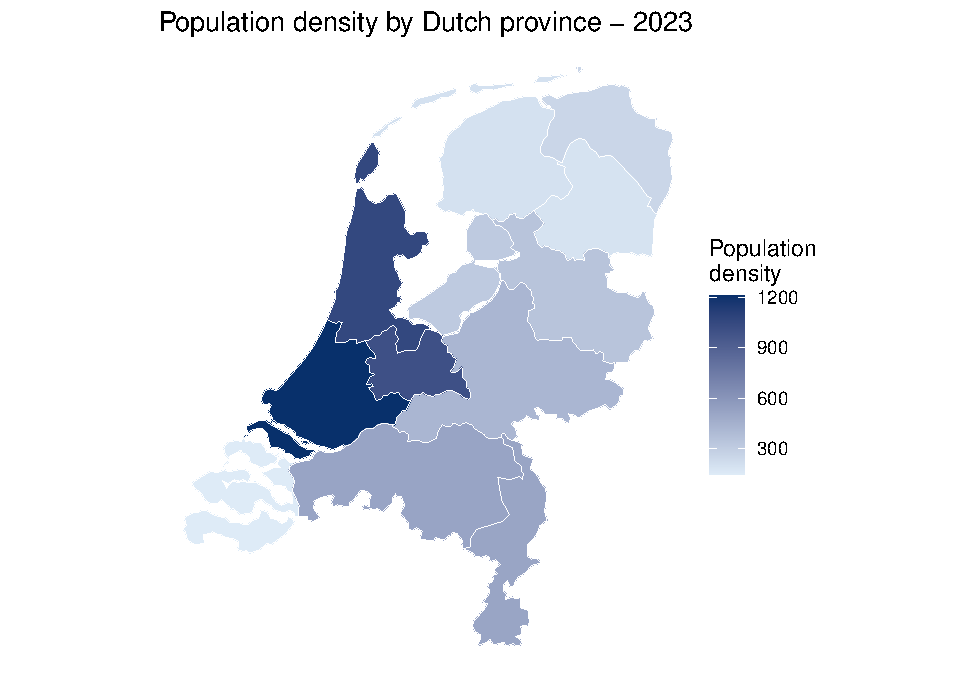
\includegraphics[keepaspectratio]{experimental-dynamic-maps_files/figure-latex/pop-heatmap-1.pdf}}

\begin{Shaded}
\begin{Highlighting}[]
\FunctionTok{ggplot}\NormalTok{(nl\_crime) }\SpecialCharTok{+}
  \FunctionTok{geom\_sf}\NormalTok{(}\FunctionTok{aes}\NormalTok{(}\AttributeTok{fill =}\NormalTok{ unemployment\_rate), }\AttributeTok{color =} \StringTok{"white"}\NormalTok{, }\AttributeTok{size =} \FloatTok{0.2}\NormalTok{) }\SpecialCharTok{+}
  \FunctionTok{scale\_fill\_gradient}\NormalTok{(}
    \AttributeTok{low  =} \StringTok{"\#e5f5e0"}\NormalTok{,  }\CommentTok{\# pale green}
    \AttributeTok{high =} \StringTok{"\#00441b"}\NormalTok{,  }\CommentTok{\# dark green}
    \AttributeTok{na.value =} \StringTok{"grey90"}\NormalTok{,}
    \AttributeTok{name =} \StringTok{"Unemployment}\SpecialCharTok{\textbackslash{}n}\StringTok{rate"}
\NormalTok{  ) }\SpecialCharTok{+}
  \FunctionTok{labs}\NormalTok{(}
    \AttributeTok{title =} \StringTok{"Unemployment rate by Dutch province – 2023"}
\NormalTok{  ) }\SpecialCharTok{+}
  \FunctionTok{theme\_minimal}\NormalTok{() }\SpecialCharTok{+}
  \FunctionTok{theme}\NormalTok{(}
    \AttributeTok{panel.grid =} \FunctionTok{element\_blank}\NormalTok{(),}
    \AttributeTok{axis.text  =} \FunctionTok{element\_blank}\NormalTok{(),}
    \AttributeTok{axis.ticks =} \FunctionTok{element\_blank}\NormalTok{()}
\NormalTok{  )}
\end{Highlighting}
\end{Shaded}

\pandocbounded{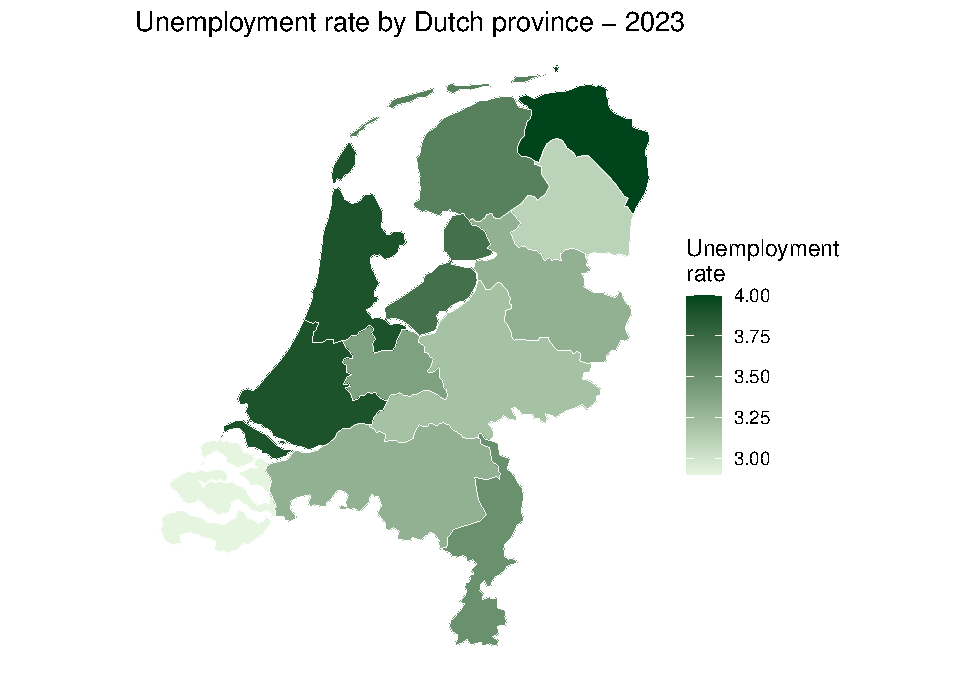
\includegraphics[keepaspectratio]{experimental-dynamic-maps_files/figure-latex/unemp-heatmap-1.pdf}}

Here you provide a description of why the plot above is relevant to your
specific social problem.

\subsection{3.5 Visualize sub-population
variation}\label{visualize-sub-population-variation}

What is the poverty rate by state?

\begin{Shaded}
\begin{Highlighting}[]
\CommentTok{\# crime}

\FunctionTok{ggplot}\NormalTok{(crime2021, }\FunctionTok{aes}\NormalTok{(}\AttributeTok{x =}\NormalTok{ leeftijdcat, }\AttributeTok{y =}\NormalTok{ crime)) }\SpecialCharTok{+}
  \FunctionTok{geom\_boxplot}\NormalTok{(}\AttributeTok{fill =} \StringTok{"yellow"}\NormalTok{, }\AttributeTok{color =} \StringTok{"black"}\NormalTok{) }\SpecialCharTok{+}
  \FunctionTok{labs}\NormalTok{(}
    \AttributeTok{title =} \StringTok{"Boxplot of Crime Suspect Rate by Age Group"}\NormalTok{,}
    \AttributeTok{x =} \StringTok{"Grouped Age Range"}\NormalTok{,}
    \AttributeTok{y =} \StringTok{"Suspects per 10,000 Inhabitants"}
\NormalTok{  ) }
\end{Highlighting}
\end{Shaded}

\pandocbounded{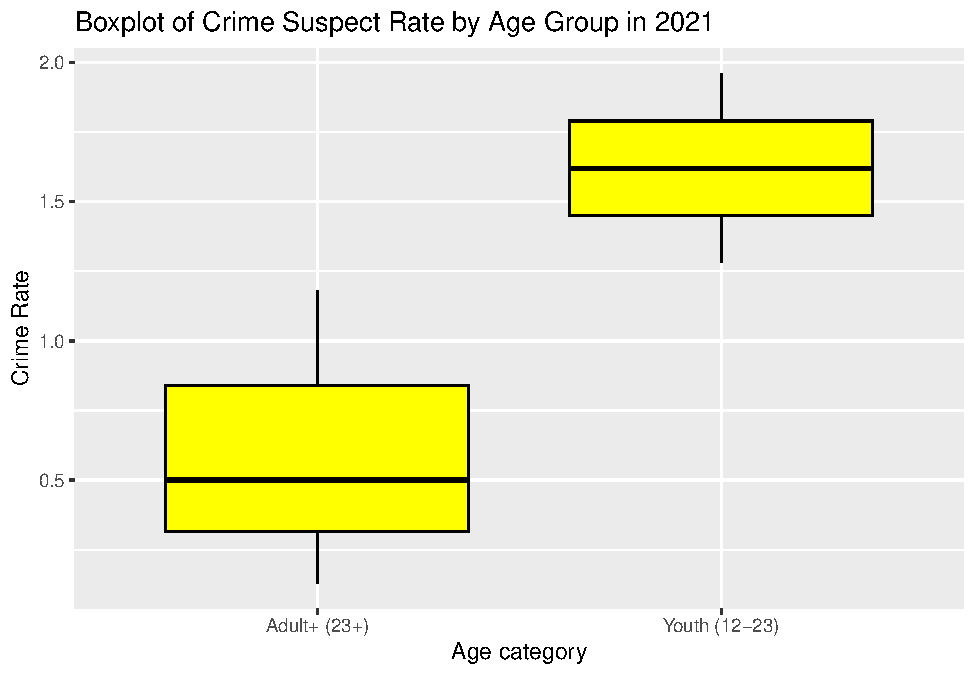
\includegraphics[keepaspectratio]{experimental-dynamic-maps_files/figure-latex/visualise_subpopulations-1.pdf}}

\begin{Shaded}
\begin{Highlighting}[]
\CommentTok{\# unemployment}

\FunctionTok{ggplot}\NormalTok{(unemployment\_age, }\FunctionTok{aes}\NormalTok{(}\AttributeTok{x =}\NormalTok{ leeftijd, }\AttributeTok{y =}\NormalTok{ unemployment)) }\SpecialCharTok{+}
  \FunctionTok{geom\_boxplot}\NormalTok{(}\AttributeTok{fill =} \StringTok{"yellow"}\NormalTok{, }\AttributeTok{color =} \StringTok{"black"}\NormalTok{) }\SpecialCharTok{+}
  \FunctionTok{labs}\NormalTok{(}
    \AttributeTok{title =} \StringTok{"Boxplot of Crime Suspect Rate by Age Group"}\NormalTok{,}
    \AttributeTok{x =} \StringTok{"Grouped Age Range"}\NormalTok{,}
    \AttributeTok{y =} \StringTok{"unemployment"}
\NormalTok{  ) }
\end{Highlighting}
\end{Shaded}

\pandocbounded{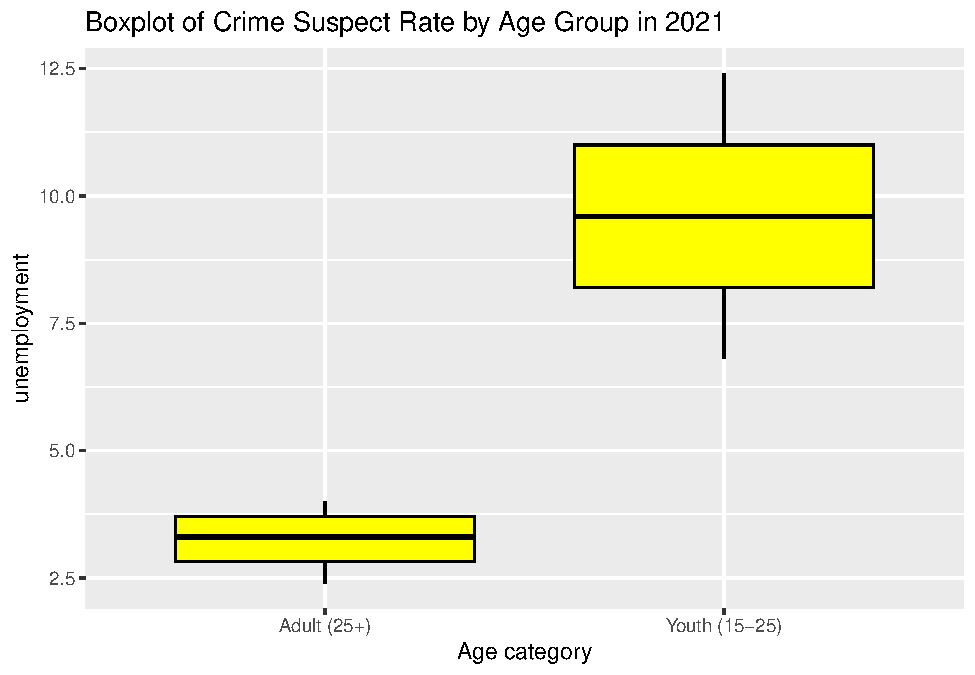
\includegraphics[keepaspectratio]{experimental-dynamic-maps_files/figure-latex/visualise_subpopulations-2.pdf}}

Here you provide a description of why the plot above is relevant to your
specific social problem.

\subsection{3.6 Event analysis}\label{event-analysis}

Analyze the relationship between two variables.

\begin{Shaded}
\begin{Highlighting}[]
\NormalTok{pivot\_agg\_data }\OtherTok{\textless{}{-}}\NormalTok{ agg\_merged }\SpecialCharTok{\%\textgreater{}\%}
  \FunctionTok{pivot\_longer}\NormalTok{(}\AttributeTok{cols =} \FunctionTok{c}\NormalTok{(unemployment, crime\_per\_capita), }\AttributeTok{names\_to =} \StringTok{"variable"}\NormalTok{, }\AttributeTok{values\_to =} \StringTok{"value"}\NormalTok{)}

\CommentTok{\# then make the plot}

\FunctionTok{ggplot}\NormalTok{(pivot\_agg\_data, }\FunctionTok{aes}\NormalTok{(}\AttributeTok{x =}\NormalTok{ year, }\AttributeTok{y =}\NormalTok{ value, }\AttributeTok{colour =}\NormalTok{ variable )) }\SpecialCharTok{+}
  \FunctionTok{geom\_line}\NormalTok{() }\SpecialCharTok{+}
  \FunctionTok{labs}\NormalTok{(}\AttributeTok{title =} \StringTok{"aggragate crime and unemployment through time"}\NormalTok{, }\AttributeTok{x =} \StringTok{"year"}\NormalTok{, }\AttributeTok{y =} \StringTok{"variable"}\NormalTok{) }\SpecialCharTok{+}
  \FunctionTok{scale\_x\_continuous}\NormalTok{(}\AttributeTok{breaks =} \FunctionTok{seq}\NormalTok{(}\DecValTok{1975}\NormalTok{, }\DecValTok{2024}\NormalTok{, }\AttributeTok{by =} \DecValTok{5}\NormalTok{), }\AttributeTok{limits =} \FunctionTok{c}\NormalTok{(}\DecValTok{1972}\NormalTok{, }\DecValTok{2026}\NormalTok{)) }\SpecialCharTok{+}
  \FunctionTok{geom\_vline}\NormalTok{(}\AttributeTok{xintercept =} \FunctionTok{c}\NormalTok{(}\DecValTok{1979}\NormalTok{, }\DecValTok{2008}\NormalTok{), }
             \AttributeTok{linetype =} \StringTok{"solid"}\NormalTok{, }
             \AttributeTok{color =} \StringTok{"black"}\NormalTok{, }
             \AttributeTok{size =} \FloatTok{0.6}\NormalTok{) }\SpecialCharTok{+} 
  \FunctionTok{annotate}\NormalTok{(}\StringTok{"text"}\NormalTok{, }\AttributeTok{x =} \DecValTok{1974}\NormalTok{, }\AttributeTok{y =} \DecValTok{9}\NormalTok{, }\AttributeTok{label =} \StringTok{"1979}\SpecialCharTok{\textbackslash{}n}\StringTok{oil{-}crisis"}\NormalTok{) }\SpecialCharTok{+}
  \FunctionTok{annotate}\NormalTok{(}\StringTok{"text"}\NormalTok{, }\AttributeTok{x =} \DecValTok{2017}\NormalTok{, }\AttributeTok{y =} \DecValTok{9}\NormalTok{, }\AttributeTok{label =} \StringTok{"2008}\SpecialCharTok{\textbackslash{}n}\StringTok{great{-}recession"}\NormalTok{)}
\end{Highlighting}
\end{Shaded}

\begin{verbatim}
## Warning: Using `size` aesthetic for lines was deprecated in ggplot2 3.4.0.
## i Please use `linewidth` instead.
## This warning is displayed once every 8 hours.
## Call `lifecycle::last_lifecycle_warnings()` to see where this warning was
## generated.
\end{verbatim}

\pandocbounded{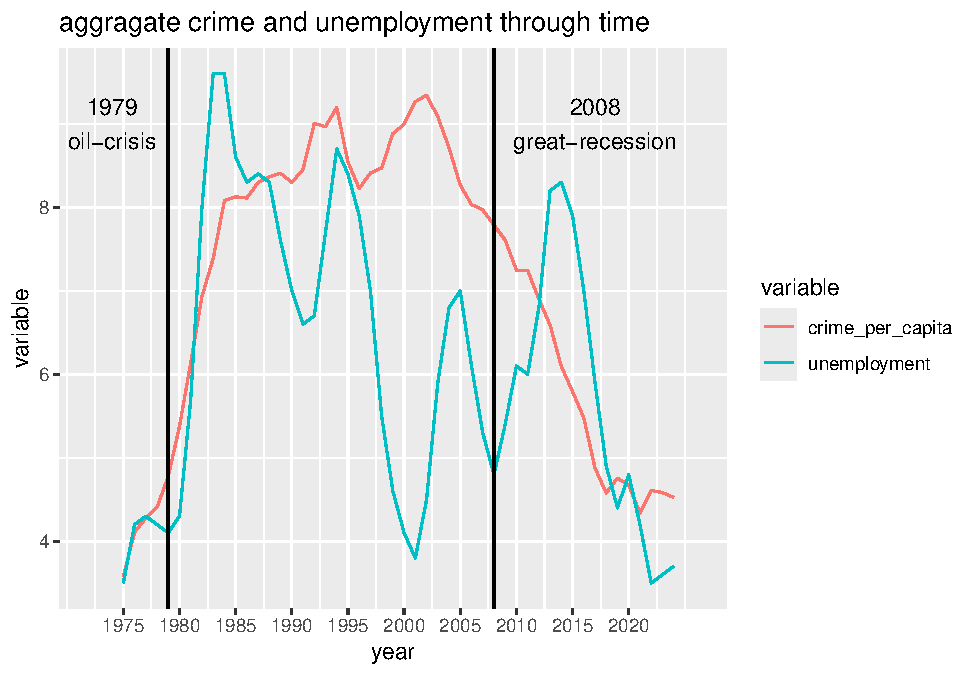
\includegraphics[keepaspectratio]{experimental-dynamic-maps_files/figure-latex/analysis-1.pdf}}

Here you provide a description of why the plot above is relevant to your
specific social problem.

\section{Part 4 - Discussion}\label{part-4---discussion}

\subsection{4.1 Discuss your findings}\label{discuss-your-findings}

\section{Part 5 - Reproducibility}\label{part-5---reproducibility}

\subsection{5.1 Github repository link}\label{github-repository-link}

Provide the link to your PUBLIC repository here: \ldots{}

\subsection{5.2 Reference list}\label{reference-list}

Use APA referencing throughout your document.

\end{document}
